\documentclass{beamer}

\usepackage[scale=2]{ccicons}
\usepackage{stmaryrd}
\usepackage{graphicx}
\usepackage{booktabs}
\usepackage{gensymb}
\usepackage{multimedia}
\usepackage{hyperref}

% Beamer configuration
\usetheme[sectionpage=progressbar, numbering=counter, progressbar=frametitle]{metropolis}

\usepackage{pgfplots}
\usepackage{pgfplotsthemetol}

% Progressbar
\setbeamercolor{progress bar}{
    fg=TolLightGreen,
    bg=TolLightGreen!50!black!30
}
\makeatletter
    \setlength{\metropolis@titleseparator@linewidth}{2pt}
    \setlength{\metropolis@progressonsectionpage@linewidth}{2pt}
    \setlength{\metropolis@progressinheadfoot@linewidth}{2pt}
\makeatother

% Footer
\setbeamertemplate{frame footer}{Quentin Brateau, ENSTA Bretagne}

% Block fill
\metroset{block=fill}

\title{Sea route monitoring by weather buoys using interval analysis}
\date{\today}
\author{Quentin Brateau}
\institute{ENSTA Bretagne}

\titlegraphic{
    \centering
    \begin{tabular}{lllll}
        \href{https://www.defense.gouv.fr/aid}{
\includegraphics[height=0.6cm]{imgs/logo_aid}} &
        \href{https://www.gdr-robotique.org/}{
\includegraphics[height=0.6cm]{imgs/logo_gdr}} &
        \href{https://www.ensta-bretagne.fr/fr/}{
\includegraphics[height=0.6cm]{imgs/logo_ensta}} &
        \href{https://labsticc.fr/fr}{
\includegraphics[height=0.6cm]{imgs/logo_labsticc}} &
        \href{https://www.ensta-bretagne.fr/robex/}{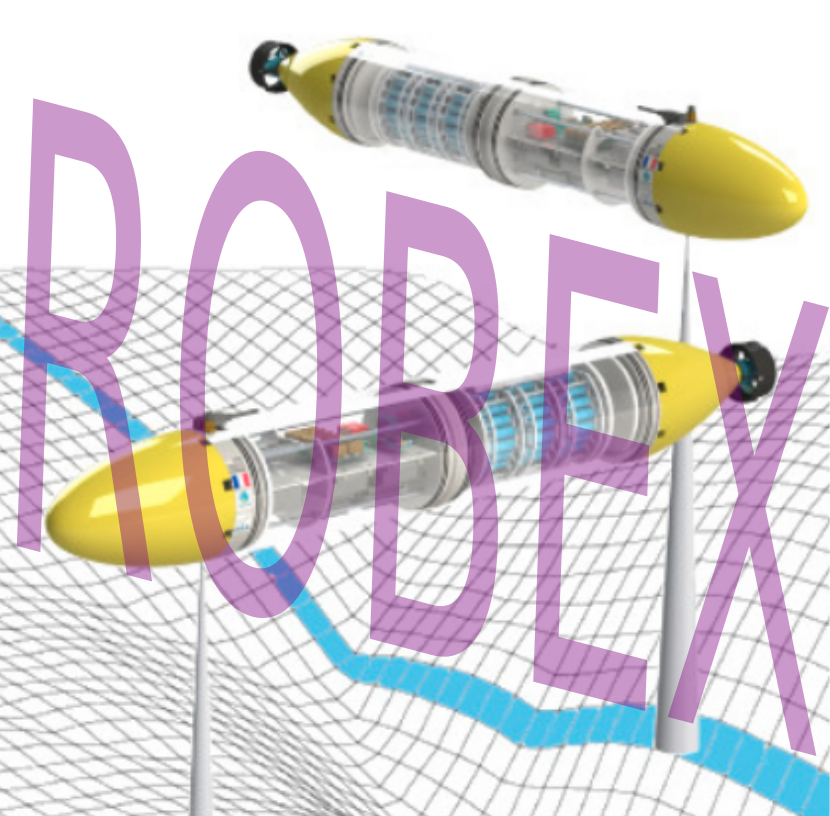
\includegraphics[height=0.6cm]{imgs/logo_robex}}
    \end{tabular}
}

\addtobeamertemplate{frametitle}{}{%
    \begin{tikzpicture}[remember picture,overlay]
    \node[anchor=north east,yshift=2pt] at (current page.north east) {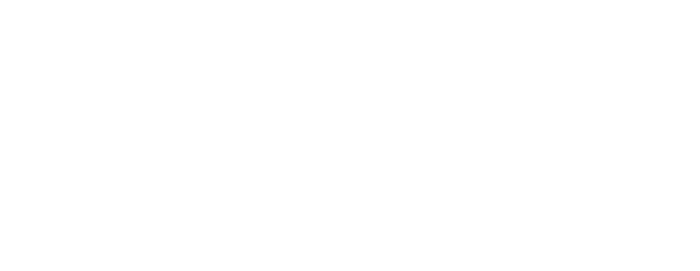
\includegraphics[height=0.9cm]{imgs/logo_ensta_bw}};
    \end{tikzpicture}
}

\begin{document}

    \maketitle
    
    \section{Time delayed detection}

        \subsection{Introduction}

            \begin{frame}{Introduction}
                \begin{minipage}{0.45\textwidth}
                    \begin{block}{Problem statement}
                        Estimate the state of a system using time delayed measurements.
                    \end{block}
                    \begin{block}{Assumptions}
                        The system emits signals at unkown time $t_i$ which are sensed at known time $t_j$.
                    \end{block}
                \end{minipage}
                \hfill
                \begin{minipage}{0.5\textwidth}
                    \begin{figure}
                        \centering
                        \href{run:introduction.mp4?autostart&loop}{\includegraphics[width=\textwidth]{build/imgs/introduction}}
                        \caption{Time delayed measurement on a system}
                    \end{figure}
                \end{minipage}
            \end{frame}

        \subsection{Formalism}

            \begin{frame}{State equation}
                \begin{block}{Evolution equation}
                    $\forall \mathbf{x} \in \mathcal{S}$ the state of the system, $\forall t \in \mathcal{T}$
                    \begin{equation}
                        \dot{\mathbf{x}}(t) = f(\mathbf{x}(t), t)
                    \end{equation}
                \end{block}

                \begin{block}{Measurement equation}
                    $\forall t_j \in \mathcal{T}$, $\exists t_i \in \mathcal{T}$ such that
                    \begin{equation}
                        g(\mathbf{x}(t_i), t_i, t_j) = 0
                    \end{equation}
                \end{block}
            \end{frame}

            \begin{frame}{Flow function}
                \begin{block}{Definition}
                    The flow function $\varphi$ is a mapping from $\mathcal{S} \times \mathcal{T} \mapsto \mathcal{S}$ such that
                    \begin{eqnarray}
                        \varphi(\mathbf{x}(t),0) &=& \mathbf{x}(t) \\
                        \varphi(\varphi(\mathbf{x}(t),t_1),t_2) &=& \varphi(\mathbf{x}(t),t_1+t_2)
                    \end{eqnarray}
                \end{block}
                \begin{block}{Property}
                    From the initial state $\mathbf{x_0} \in \mathcal{S}$, $\forall t \in \mathcal{T}$
                    \begin{eqnarray}
                        \varphi(\mathbf{x_0},t) &=& \mathbf{x}(t) \\
                        \varphi(\mathbf{x}(t),-t) &=& \mathbf{x}_0
                    \end{eqnarray}
                \end{block}
            \end{frame}

            \begin{frame}{State estimation}
                \begin{block}{Compatible set}
                    $\mathbb{C}_{t_j}$ is the set of compatible state with measurement at $t_j$ such that $\forall t_j \in \mathcal{T}$
                    \begin{eqnarray}
                        \mathbb{C}_{t_j} = \{ (\mathbf{x}, t_i) \in \mathcal{S} \times \mathcal{T} \mid g(\mathbf{x}(t_i), t_i, t_j) = 0\}
                    \end{eqnarray}
                \end{block}

                \begin{block}{Initial state estimation}
                    Using the \textbf{flow function}, $\mathbb{X}_0$ is the estimated state of the system
                    \begin{eqnarray}
                        \mathbb{X}_0 = \{ \mathbf{x_0} \in \mathcal{S} \mid \exists (\mathbf{x}, t_i) \in \mathbb{C}_{t_j}, \mathbf{x_0} = \varphi(\mathbf{x}(t_i), -t_i) \}
                    \end{eqnarray}
                \end{block}
            \end{frame}
    
    \section{Application: Boat wakes}

            \begin{frame}{Introduction}
                \begin{figure}
                    \centering
                    \href{run:boat.mp4?autostart&loop}{\includegraphics[width=0.52\textwidth]{build/imgs/boat}}
                    \caption{Boat's wake detection}
                \end{figure}
            \end{frame}

            \begin{frame}{Application: Boat's wakes}
                \begin{block}{Boat's state}
                    The system is a boat moving straight ahead along the x-axis
                    $$\mathbf{x} = (x, y, v)^T$$ 
                \end{block}
                \begin{block}{State space assumptions}
                    \begin{equation}
                    \begin{cases}x \in [x_{min}, x_{max}] \\ y \in [y_{min}, y_{max}] \\ v \in [-v_{max}, -v_{min}] \cup [v_{min}, v_{max}] \end{cases}
                    \end{equation}
                \end{block}
            \end{frame}

            \begin{frame}{State equations}
                \begin{block}{Evolution equation}
                    \begin{equation}
                        \begin{aligned}
                            f\colon \mathcal{S} &\to \mathcal{S} \\
                            \mathbf{x} &\mapsto (v.dt, 0, 0)^T
                        \end{aligned}
                    \end{equation}
                \end{block}
                \begin{block}{Flow function}
                    \begin{equation}
                        \begin{aligned}
                            \varphi\colon \mathcal{S} \times \mathcal{T} &\to \mathcal{S} \\
                            (\mathbf{x}, t) &\mapsto (x + v.t, y, v)^T
                        \end{aligned}
                    \end{equation}
                \end{block}
            \end{frame}

            \begin{frame}{State equations}
                \begin{block}{Measurement function}
                    \begin{equation}
                        \begin{aligned}
                            g\colon \mathcal{S} \times \mathcal{T} \times \mathcal{T} &\to \mathcal{T} \\
                            (\mathbf{x}(t_i), t_i, t_j) &\mapsto sec(\alpha) \cdot |y - y_s| - v \cdot sin(\alpha) \cdot (t_j - t_i)
                        \end{aligned}
                    \end{equation}
                \end{block}
                \begin{block}{Detection condition}
                    \begin{itemize}
                        \item Wake's velocity vector aligned with boat-sensor's vector \\
                        \item Traveled distance between boat and sensor equal to the wake's velocity times the time difference
                    \end{itemize}
                \end{block}
            \end{frame}

            \begin{frame}{Application}
                \begin{minipage}{0.45\textwidth}
                    \begin{figure}
                            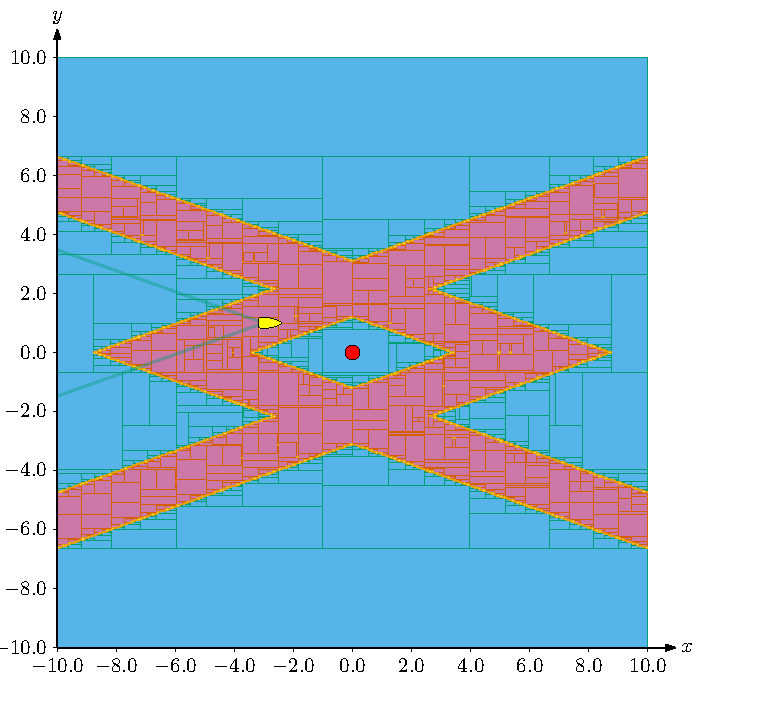
\includegraphics[width=\textwidth]{imgs/forward}
                            \caption{Forward boat detection set $\mathbb{Y}_1^1 = \lbrack3.38, 4.38\rbrack s$}
                    \end{figure}
                \end{minipage}
                \hfill
                \begin{minipage}{0.45\textwidth}
                    \begin{figure}
                            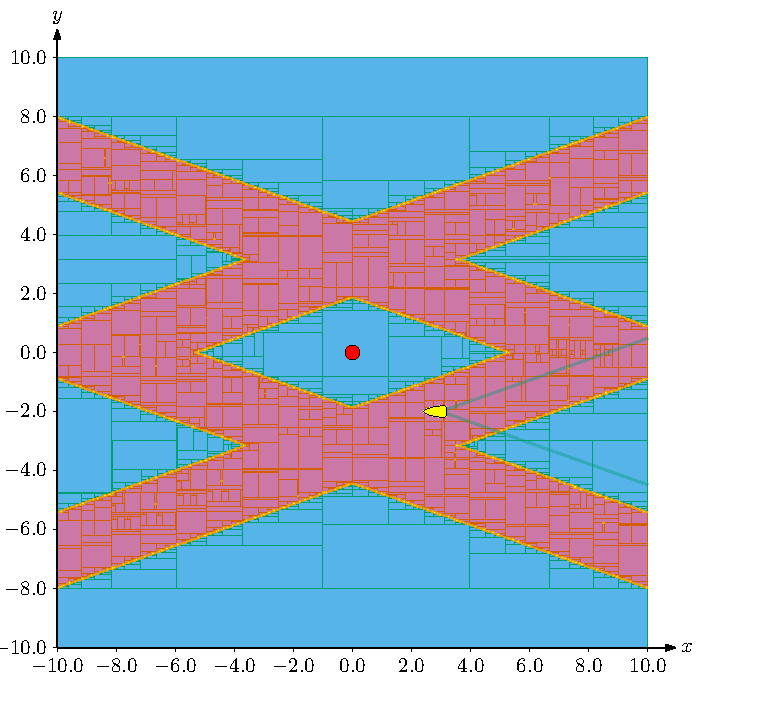
\includegraphics[width=\textwidth]{imgs/backward}
                            \caption{Backward boat detection set $\mathbb{Y}_1^1 = \lbrack5.26, 6.26\rbrack s$}
                    \end{figure}
                \end{minipage}
            \end{frame}
            

    \section{More systems, more sensors}

        \subsection{Introduction}

            \begin{frame}{Introduction}
                \begin{block}{Problem statement}
                    Estimate the state of multiples sub-systems governed by the same \textbf{evolution equation}.
                \end{block}
                \begin{block}{Measurements}
                    Measurements are \textbf{indistinguishable}. Sub-systems are sensed by \textbf{independant} sensors. The number of sensors can be significant.
                \end{block}
            \end{frame}

            \subsection{Combinatorial approach}

            \begin{frame}{Combinatorial approach}
                \begin{block}{Combinatorial approach}
                    $\forall l \in \mathbb{N}$ the number of sub-systems, $\forall m \in \mathbb{N}$ the number of sensors, there is $d = l^m$ detections.
                \end{block}
                \begin{exampleblock}{Example}
                    With $l = 5$ boats and $m = 20$ sensors,
                    $$d = l^m = 5^{20} \simeq 9.5e^{13}$$
                \end{exampleblock}
            \end{frame}

        \subsection{Proposed approach}

            \begin{frame}{Proposed approach}
                \begin{block}{Rules}
                    \begin{itemize}
                        \item Any detection could be produced by any sub-system.
                        \item Estimate possible states for all sub-systems at once.
                    \end{itemize}
                \end{block}
                \begin{block}{Advantages}
                    Processing the union of all measurements for a sensor as one set to avoid the \textbf{combinatorial aspect}.
                \end{block}
            \end{frame}

            \begin{frame}{Proposed approach}
                \begin{block}{Proposed approach}
                    $\forall l \in \mathbb{N}$ the number of sub-systems, $\forall m \in \mathbb{N}$ the number of sensors, there is $d = l \times m$ detections.
                \end{block}
                \begin{exampleblock}{Example}
                    With $l = 5$ boats and $m = 20$ sensors,
                    $$d = l \times m = 5 \times 20 = 120$$
                \end{exampleblock}
            \end{frame}

        \subsection{Detection space}

            \begin{frame}{Detection space}
                \begin{block}{Sensor detection set}
                    $\forall k \in \llbracket 1, m\rrbracket$, $\mathbb{Y}^k$ is the detection set of the $k^{th}$ sensor such that
                    \begin{equation}
                        \mathbb{Y}^k = \bigcup_{j \in \llbracket 1, l\rrbracket} \mathbb{Y}_j^k
                    \end{equation}
                \end{block}
                \begin{block}{Detection set}
                    The detection set is a subset of $\mathbb{R}^m$, and $\mathbb{Y}$ is the detection set of all the systems such that
                    \begin{equation}
                        \mathbb{Y} = \mathbb{Y}^1 \times \dots \times \mathbb{Y}^m
                    \end{equation}
                \end{block}
            \end{frame}

            \begin{frame}{Example}
                \begin{exampleblock}{Example}
                    Assuming that $n = 3$, $m = 2$, and
                    $$\forall k \in \llbracket 1, m\rrbracket, \;  \forall j \in \llbracket 1, l\rrbracket, \quad \mathbb{Y}_j^k \in \mathbb{IR}$$
                \end{exampleblock}
                \begin{exampleblock}{Detection space}
                    Then $\mathbb{Y} \in \mathbb{IR}^2$ and
                    \begin{eqnarray}
                        \mathbb{Y} & = & \mathbb{Y}^1 \times \mathbb{Y}^2 \\
                        & = & \left(\mathbb{Y}_1^1 \cup \mathbb{Y}_2^1 \cup \mathbb{Y}_3^1\right) \times \left(\mathbb{Y}_1^2 \cup \mathbb{Y}_2^2 \cup \mathbb{Y}_3^2\right)
                    \end{eqnarray}
                \end{exampleblock}
            \end{frame}

            \begin{frame}{Example}
                \begin{minipage}{0.45\textwidth}
                    \begin{table}
                        \begin{tabular}{@{} rcc @{}}
                            \toprule
                            & $k=1$ & $k=2$ \\
                            \midrule
                            $\mathbb{Y}_1^k$ & $\lbrack0.97, 1.97\rbrack$ & $\lbrack1.51, 2.51\rbrack$  \\
                            $\mathbb{Y}_2^k$ & $\lbrack3.18, 4.18\rbrack$ & $\lbrack4.01, 1.01\rbrack$ \\
                            $\mathbb{Y}_3^k$ & $\lbrack6.62, 7.62\rbrack$ & $\lbrack6.47, 6.47\rbrack$ \\
                            \bottomrule
                        \end{tabular}
                        \caption{Detection times}
                    \end{table}
                \end{minipage}
                \hfill
                \begin{minipage}{0.5\textwidth}
                    \begin{figure}
                        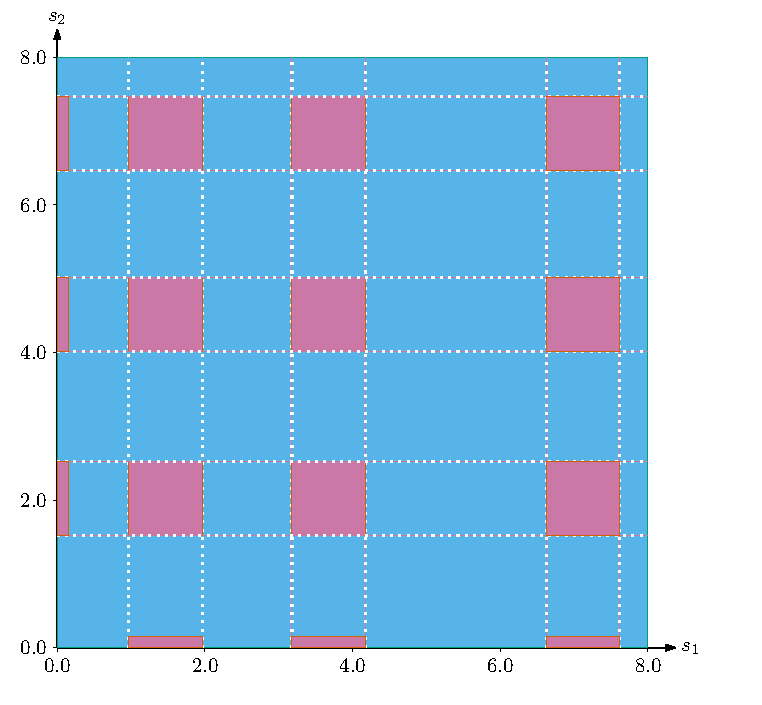
\includegraphics[height=0.7\textheight]{imgs/detection_space}
                        \caption{Detection space}
                    \end{figure}
                \end{minipage}
            \end{frame}

    \section{Application: Sea route monitoring}

        \subsection{Formalism}
            
            \begin{frame}{State estimation}
                \begin{block}{Compatible set}
                    $\mathbb{C}$ is the set of compatible state with measurements such that
                    \begin{eqnarray}
                        \mathbb{C} = \{ (\mathbf{x}, t_i) \in \mathcal{S} \times \mathcal{T} \mid \forall t_j \in \mathbb{Y}, g(\mathbf{x}(t_i), t_i, t_j) = 0\}
                    \end{eqnarray}
                \end{block}

                \begin{block}{Initial state estimation}
                    Using the \textbf{flow function}, $\mathbb{X}_0$ is the estimated state of the system
                    \begin{eqnarray}
                        \mathbb{X}_0 = \{ \mathbf{x_0} \in \mathcal{S} \mid \exists (\mathbf{x}, t_i) \in \mathbb{C}, \mathbf{x_0} = \varphi(\mathbf{x}(t_i), -t_i) \}
                    \end{eqnarray}
                \end{block}
            \end{frame}

        \subsection{Example: two sensors and three boats}

            \begin{frame}{Example: two sensors and three boats}
                \begin{minipage}{0.45\textwidth}
                    \begin{figure}
                            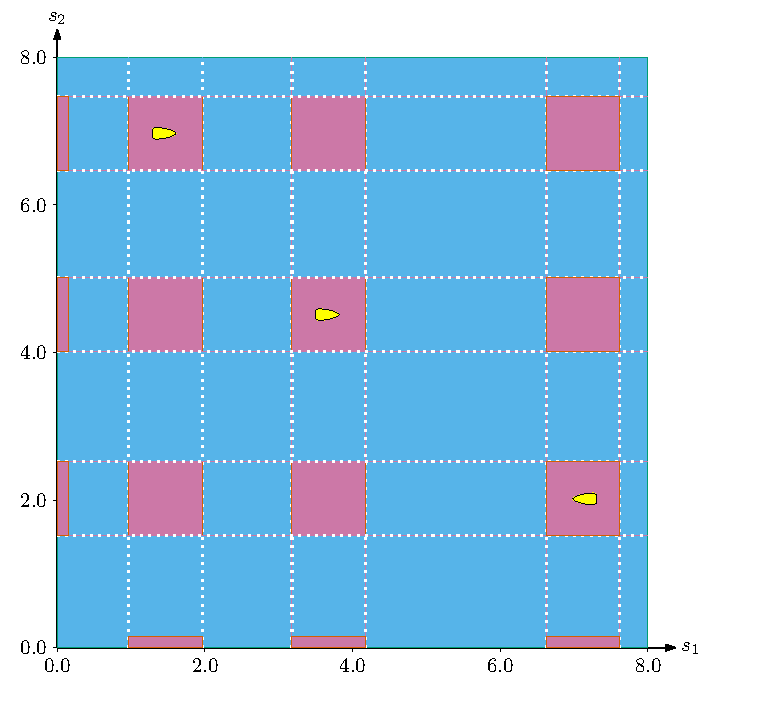
\includegraphics[width=\textwidth]{imgs/ex_detection_space}
                            \caption{Detection space}
                    \end{figure}
                \end{minipage}
                \hfill
                \begin{minipage}{0.45\textwidth}
                    \begin{figure}
                            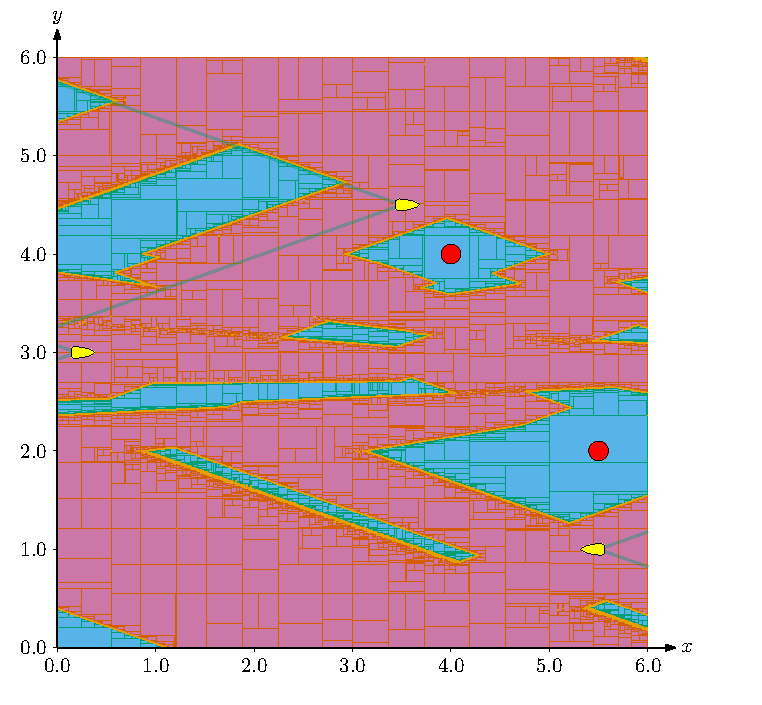
\includegraphics[width=\textwidth]{imgs/ex_boat_space}
                            \caption{Boat space}
                    \end{figure}
                \end{minipage}
            \end{frame}

        \subsection{Causal approach}

            \begin{frame}{Causal approach}
                \begin{figure}
                    \centering
                    \href{run:causal.mp4?autostart}{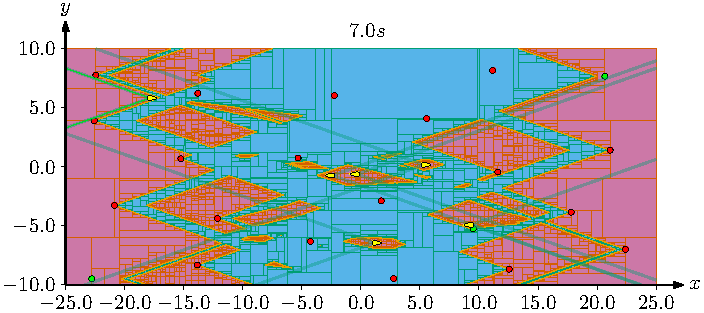
\includegraphics[width=\textwidth]{imgs/causal_cover}}
                    \caption{Causal simulation}
                \end{figure}
            \end{frame}

            \begin{frame}{Causal approach - Focus}
                \begin{figure}
                    \centering
                    \vspace{0.2cm}
                    \begin{overprint}
                        \onslide<1>\href{run:focus_1.mp4?loop}{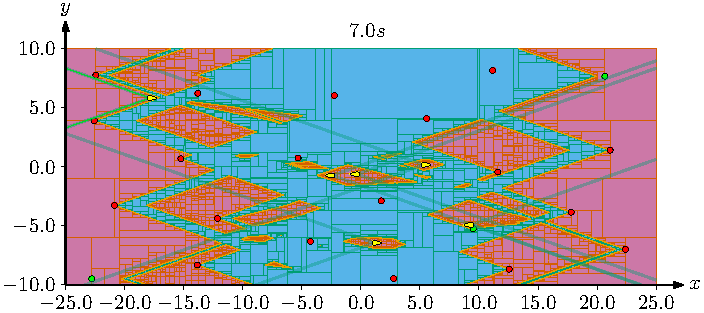
\includegraphics[width=\textwidth]{imgs/focus_1}}
                            \caption{Causal simulation - Outliers}

                        \onslide<2>\href{run:focus_2.mp4?loop}{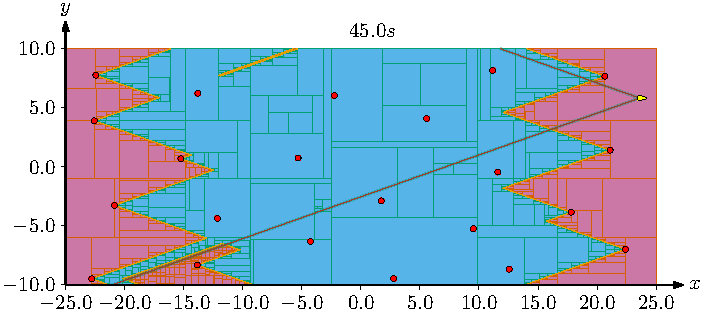
\includegraphics[width=\textwidth]{imgs/focus_2}}
                            \caption{Causal simulation - Two side detection}
                    \end{overprint}
                \end{figure}
            \end{frame}

        \subsection{Acausal approach}

            \begin{frame}{Acausal approach}
                \begin{figure}
                    \centering
                    \href{run:acausal.mp4?autostart}{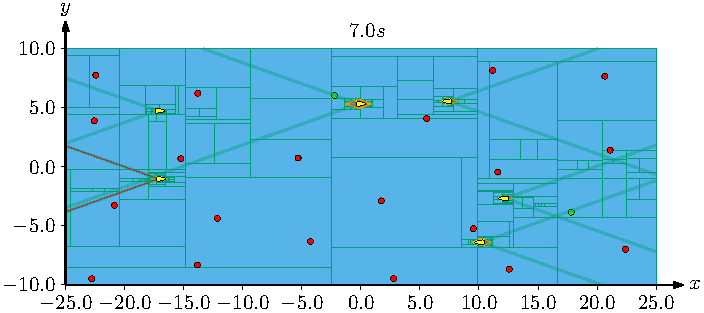
\includegraphics[width=\textwidth]{imgs/acausal_cover}}
                    \caption{Acausal simulation}
                \end{figure}
            \end{frame}

            

            % \begin{frame}{Formalism}
            %     \begin{figure}
            %         \centering
            %         \includegraphics[width=0.6\textwidth]{build/imgs/space_time}
            %         \caption{Space time state estimation}
            %     \end{figure}
            % \end{frame}


    % \section{Introduction}

    %     \subsection{Problem statement}

            

        

    % \section{Formalism}

    %     \subsection{State equation}

    %         \begin{frame}{State equation}
    %             \begin{block}<1->{Evolution equation}
    %                 $\forall l \in \mathbb{N}$ the number of sub-systems, $\forall i \in \llbracket 1, l\rrbracket$, $\mathbf{x_i} \in \mathbb{R}^n$ is the state of the $i^{th}$ system such that
    %                 \begin{equation}
    %                     \dot{\mathbf{x_i}} = f(\mathbf{x_i})
    %                 \end{equation}
    %             \end{block}

    %             \begin{block}<2->{Measurement equation}
    %                 $\forall m \in \mathbb{N}$ the number of sensors, $\forall k \in \llbracket 1, m\rrbracket$, $\exists j \in \llbracket 1, l\rrbracket$ such that
    %                 \begin{equation}
    %                     g^k(\mathbf{x_i}(t_j)) \in \mathbb{Y}_j^k
    %                 \end{equation}
    %             \end{block}
    %         \end{frame}

        

    % \section{Detection space}

        

    % \section{State space}

    %     \subsection{State space}

    %         \begin{frame}{State space}
    %             \begin{block}<1->{State space}
    %                 The state space is a subset of $\mathbb{R}^n$ and the state of the system is estimated using set inversion algorithm.
    %                 \begin{equation}
    %                     \mathbb{X} = \lbrace \mathbf{x} \in \mathbb{R}^n \mid\ g(\mathbf{x}) \in \mathbb{Y}\rbrace
    %                 \end{equation}
    %             \end{block}
    %         \end{frame}

    % \section{Summary}

    %     \subsection{Summary}

    %     \begin{frame}{Summary}
    %         \begin{figure}
    %             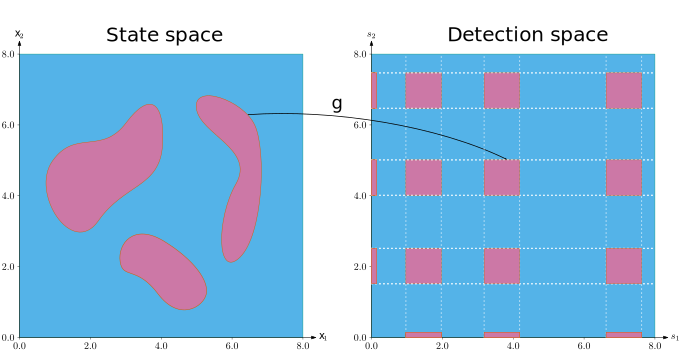
\includegraphics[width=\textwidth]{build/imgs/formalism}
    %             \caption{Summary of the formalism}
    %         \end{figure}
    %     \end{frame}

    

            % \begin{frame}{Introduction}
            %     \begin{minipage}[b]{0.55\textwidth}
            %         \begin{block}<1->{Sea route monitoring}
            %             Many applications
            %             \begin{itemize}
            %                 \item Traffic safety
            %                 \item Surveillance operations
            %                 \item Intruder detection
            %             \end{itemize}
            %         \end{block}
            %         \begin{block}<2->{Weather buoys}
            %             \begin{itemize}
            %                 \item Deployed all over the world\footnotemark[1]
            %                 \item Disturbed by boat's wake
            %             \end{itemize}
            %         \end{block}
            %     \end{minipage}
            %     \hfill
            %     \begin{minipage}[b]{0.4\textwidth}
            %         \onslide<2->
            %         \begin{figure}
            %             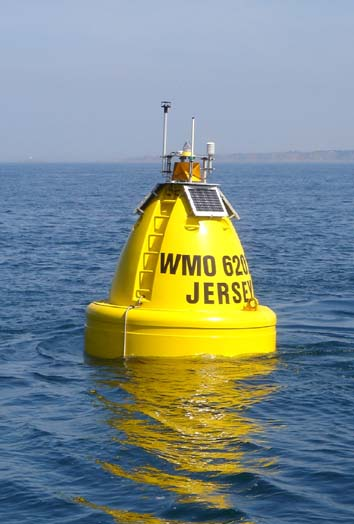
\includegraphics[width=0.8\textwidth, trim={0, 50, 0, 50}, clip]{imgs/buoy}
            %             \caption{Weather buoy - NOAA\footnotemark[1]}
            %         \end{figure}
            %     \end{minipage}

            %     \footnotetext[1]{{\url{https://www.ndbc.noaa.gov/}}}
            % \end{frame}

        % \subsection{Boat wake}

        %     \begin{frame}{Boat wake}
        %         \centering
        %         \begin{minipage}{0.6\textwidth}
        %             \begin{block}{Wake's angle}
        %                 \begin{equation}
        %                     \alpha = \arcsin\left(\frac{1}{3}\right) \approx 19.47 \degree
        %                 \end{equation}
        %             \end{block}
        %             \vspace{0.2cm}
        %             \begin{figure}
        %                 \centering
        %                 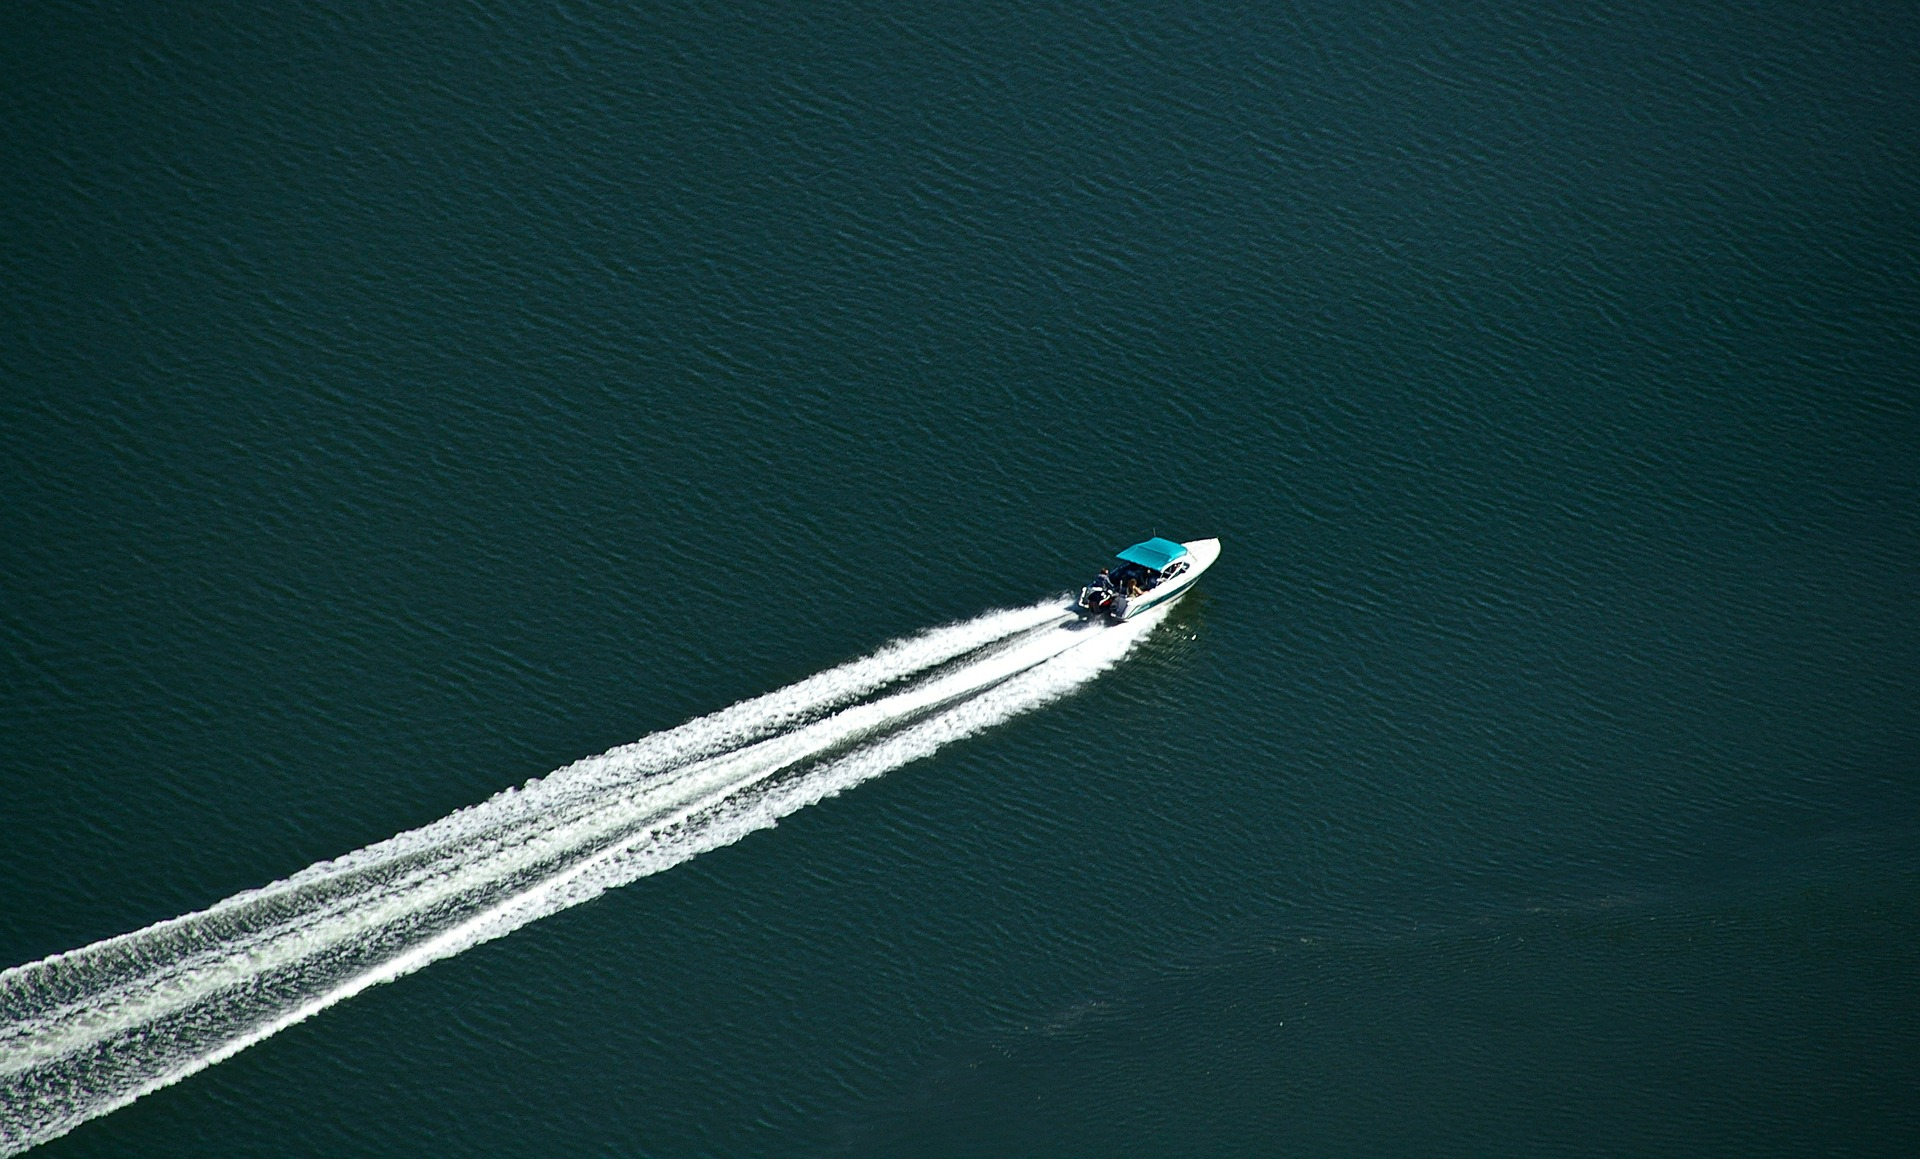
\includegraphics[width=\textwidth,trim={0 0 17cm 14cm},clip]{imgs/motorboat}
        %                 \caption{Boat and wake}
        %             \end{figure}
        %         \end{minipage}
        %     \end{frame}
        
        % \subsection{Formalism}

        %     \begin{frame}{Formalism}
        %         \begin{block}<1->{Boat's state}
        %             Assuming each boats are moving straight ahead along the x-axis
        %             $$\forall i \in \llbracket 1, n\rrbracket, \quad \mathbf{x_i} = (x_i, y_i, v_i)^T$$ 
        %         \end{block}

        %         \begin{block}<2->{State equation}
        %             \begin{eqnarray}
        %                 f:& \mathbf{x_i} &\mapsto (v_i.dt, 0, 0)^T \\
        %                 g^k:& \mathbf{x_i}  &\mapsto \frac{1}{v_i} \left(\frac{\lvert y_i - y^k \rvert}{tan(\alpha)} - (x_i - x^k)\right)
        %             \end{eqnarray}
        %         \end{block}
        %     \end{frame}

        %     \begin{frame}{Assumptions}
        %         \begin{block}<1->{Boat's state}
        %             We will consider a state space, such that
        %             \begin{equation}
        %                 \forall i \in \llbracket 1, n\rrbracket, \quad \begin{cases}x_i \in [x_{min}, x_{max}] \\ y_i \in [y_{min}, y_{max}] \\ v_i \in [-v_{max}, -v_{min}] \cup [v_{min}, v_{max}] \end{cases}
        %             \end{equation}
        %         \end{block}
        %         \begin{block}<2->{Sensor's data}
        %             \begin{itemize}
        %                 \item Causal simulation
        %                 \item Acausal simulation
        %             \end{itemize}
        %         \end{block}
        %     \end{frame}
        
        % \subsection{Example: single sensor and single boat}

        %     \begin{frame}{Example: single sensor and single boat}
        %         \begin{minipage}{0.45\textwidth}
        %             \begin{figure}
        %                     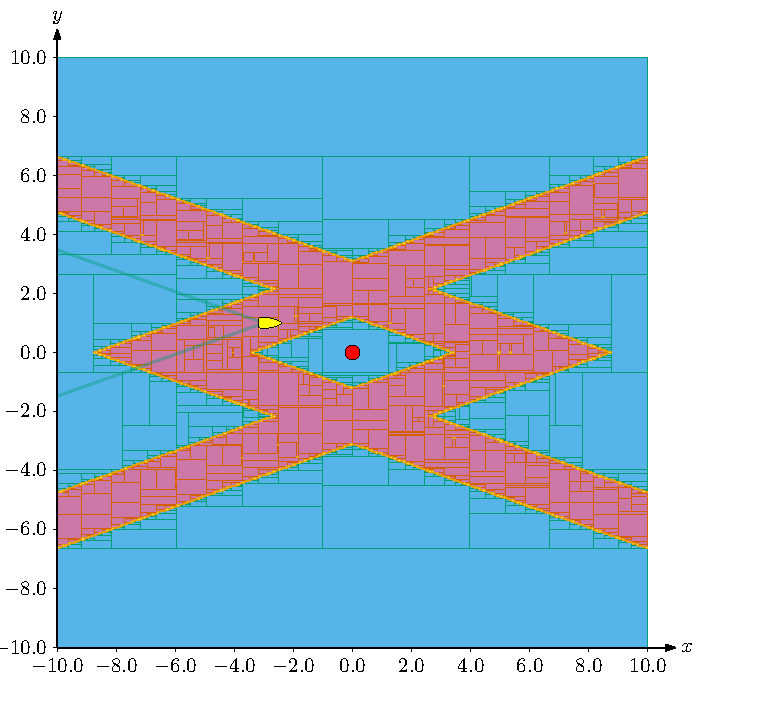
\includegraphics[width=\textwidth]{imgs/forward}
        %                     \caption{Forward boat detection set $\mathbb{Y}_1^1 = \lbrack3.38, 4.38\rbrack s$}
        %             \end{figure}
        %         \end{minipage}
        %         \hfill
        %         \begin{minipage}{0.45\textwidth}
        %             \begin{figure}
        %                     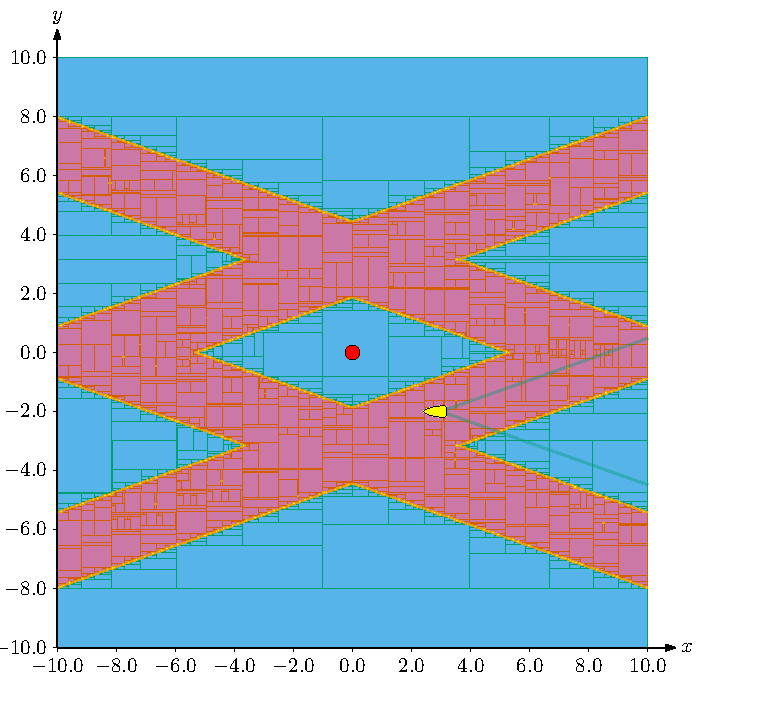
\includegraphics[width=\textwidth]{imgs/backward}
        %                     \caption{Backward boat detection set $\mathbb{Y}_1^1 = \lbrack5.26, 6.26\rbrack s$}
        %             \end{figure}
        %         \end{minipage}
        %     \end{frame}

        

    \section{Conclusion}

        \subsection{Conclusion}

            \begin{frame}{Conclusion}
                \centering
                \begin{minipage}{0.8\textwidth}
                    \begin{block}{Proposed approach}
                        Consider the set of measurements together to estimate the state of sub-systems at once.
                    \end{block}
                    \begin{block}{Benefits}
                        Deal with \textbf{large-scale} problems without combinatorial complexity.
                    \end{block}
                    \begin{block}{Limitations}
                        No individual state estimation for each sub-systems and the result possibly contains outliers.
                    \end{block}
                \end{minipage}
            \end{frame}

        \subsection{Outlook}

            \begin{frame}{Outlook}
                \centering
                \begin{minipage}{0.8\textwidth}
                    \begin{block}{Further work}
                        \vspace{0.25cm}
                        \begin{itemize}
                            \item Count the number of boats
                            \item Take off associated measurements related to a sub-system
                            \item Characterize the set of outliers to hide sub-systems from sensors
                        \end{itemize}
                    \end{block}
                \end{minipage}
            \end{frame}
    
    \appendix

    \begin{frame}[standout]
        Questions?
    \end{frame}
    
\end{document}